
It is desirable for a depth function $D\colon \R^d \times \mathscr{F} \to \R$
to satisfy the following properties, described by
\textcite{zuo-serfling-2000}.

\begin{enumerate}
    \item[\textbf{P1}.] \emph{Affine invariance.}
        For any random vector $\vX$ in $\R^d$, any $d \times d$ nonsingular
        matrix $A$, and any $d$-vector $\bm{b}$,
        \begin{equation}
            D(A\vx + \bm{b}, F_{A\vX + \bm{b}}) \;=\; D(\vx, F_{\vX}).
        \end{equation}
        This makes $D(\vX, F_{\vX})$ independent of the choice of coordinate
        system.

    \item[\textbf{P2}.] \emph{Maximality at center.}
        For any $F \in \mathscr{F}$ having `center' $\vth$,
        \begin{equation}
            D(\vth, F) \;=\; \sup_{\vx \in \R^d} D(\vx, F).
        \end{equation}
        This means that the deepest point coincides with some center of
        symmetry of the distribution $F$.

    \item[\textbf{P3}.] \emph{Monotonicity relative to deepest point.}
        For any $F \in \mathscr{F}$ having deepest point $\vth$ and for
        $\alpha \in [0, 1]$,
        \begin{equation}
            D(\vx, F) \;\leq\; D(\vth + \alpha(\vx - \vth), F).
        \end{equation}
        Thus, $D(\Cdot, F)$ monotonically decreases along any ray pointing
        away from the deepest point.

    \item[\textbf{P4}.] \emph{Vanishing at infinity.}
        For any $F \in \mathscr{F}$,
        \begin{equation}
            D(\vx, F) \to 0 \quad\text{ as }\quad\norm{\vx} \to \infty.
        \end{equation}
\end{enumerate}

Furthermore, we demand that $D$ be non-negative and bounded.
Thus, we may assume hereon that $D$ only takes values in $[0, 1]$.

The notion of a `center' of a distribution in \textbf{P2} is typically
described in terms of symmetry.
We say that a random vector $\vX$ is \emph{centrally symmetric} about
$\vth \in \R^d$ if $\vX - \vth \eqd \vth - \vX$.
Similarly, we say that $\vX$ is \emph{angularly symmetric} about $\vth$ if
$(\vX - \vth) / \norm{\vX - \vth}$ is centrally symmetric about $\bm0$.
An even more restrictive notion of symmetry is \emph{spherical symmetry},
where we demand that $U(\vX - \vth) \eqd \vX - \vth$ for every orthonormal
matrix $U$.
\emph{Elliptical symmetry} requires that $V\vX$ is spherically symmetric about
$\vth$ for some nonsingular matrix $V$.
Finally, the weakest notions of symmetry discussed here is \emph{halfspace
symmetry}, where we impose $P(\vX \in H) \geq 1/2$ for every closed halfspace
in $\R^d$ containing $\vth$.
Thus, the symmetries in decreasing order of strength are $S > E > C > A > H$.


\section{Depth contours}
\label{sec:multivariate_depthcontours}

Given a depth function $D$ and some fixed distribution $F \in \mathscr{F}$, we
may examine contours produced by $D(\Cdot, F)$.
The following definitions are adapted from \cite{liu-parelius-singh-1999}.

\begin{definition}
    The contour of depth $t$ is the set $\{\vx \in \R^d : D(\vx, F) = t\}$.
\end{definition}

\begin{definition}
    The region enclosed by the contour of depth $t$ is the set
    \begin{equation}
        R_F(t) \,=\, \{\vx \in \R^d : D(\vx, F) > t\}.
    \end{equation}
\end{definition}

It is often more convenient to deal with depth contours and regions based on
their probability content rather than a depth cutoff.

\begin{definition}
    The $p$-th central region is the set
    \begin{equation}
        C_F(p) \,=\, \bigcap_{t}\; \{R_F(t) : P_F(R_F(t)) \geq p\}.
    \end{equation}
\end{definition}

\begin{definition}
    The $p$-th level contour, or center-outward contour surface, is the set
    $Q_F(p) = \partial C_F(p)$.
\end{definition}


\begin{example}
    Consider $\UU(B^d)$, i.e.\ the uniform distribution on the unit ball in
    $\R^d$.
    While there are no proper density contours to speak of, halfspace depth
    contours are concentric spheres centered at the origin, the deepest point.
    This illustrates how depth contours are more suited to indicating
    centrality than density contours.
\end{example}


\begin{definition}
    Let $\vX_1, \dots, \vX_n \iid F$.
    We introduce depth based order statistics $\vX_{[1]}, \dots, \vX_{[n]}$,
    which are a reordering of the sample in decreasing order of depth, i.e.\
    $D(\vX_{[1]}, F) \geq \dots \geq D(\vX_{[n]}, F)$.
\end{definition}

With this, given $\vX_1, \dots, \vX_n \iid F$, the sample $p$-th central
region is given by
\begin{equation}
    C_{\hat{F}_n}(p) = \conv(\vX_{[1]}, \dots, \vX_{[\lceil np \rceil]}).
\end{equation}


\section{Depth-Depth plots}

\begin{definition}[DD plot] \label{def:ddplot}
    Let $F, G$ be two distributions on $\R^d$, and let $D$ be a depth
    function. The Depth-Depth plot, also known as the DD plot, of $F$ and $G$
    is given by
    \begin{equation}
        \DD(F, G) \,=\, \{(D(\vz, F), D(\vz, G)) : \vz \in \R^d\}.
    \end{equation}
\end{definition}
\begin{remark}
    The above definition generalizes naturally to involve more than two
    distributions on $\R^d$.
\end{remark}

When the depth function $D$ only takes values in $[0, 1]$, the DD plot is a
subset of $[0, 1]^2$ and hence easily visualized.
Clearly when $F = G$, the corresponding DD plot is confined to the diagonal
$\{(t, t) : t \in [0, 1]\}$.
However, when $d \geq 2$ and $F, G$ are absolutely continuous, $\DD(F, G)$ has
non-zero area (Lebesgue measure) when $F \neq G$.
Assuming that $D$ is affine invariant, \textcite{liu-parelius-singh-1999}
propose this area as an affine invariant measure of the discrepancy between
$F$ and $G$.



\begin{figure}
    \centering
    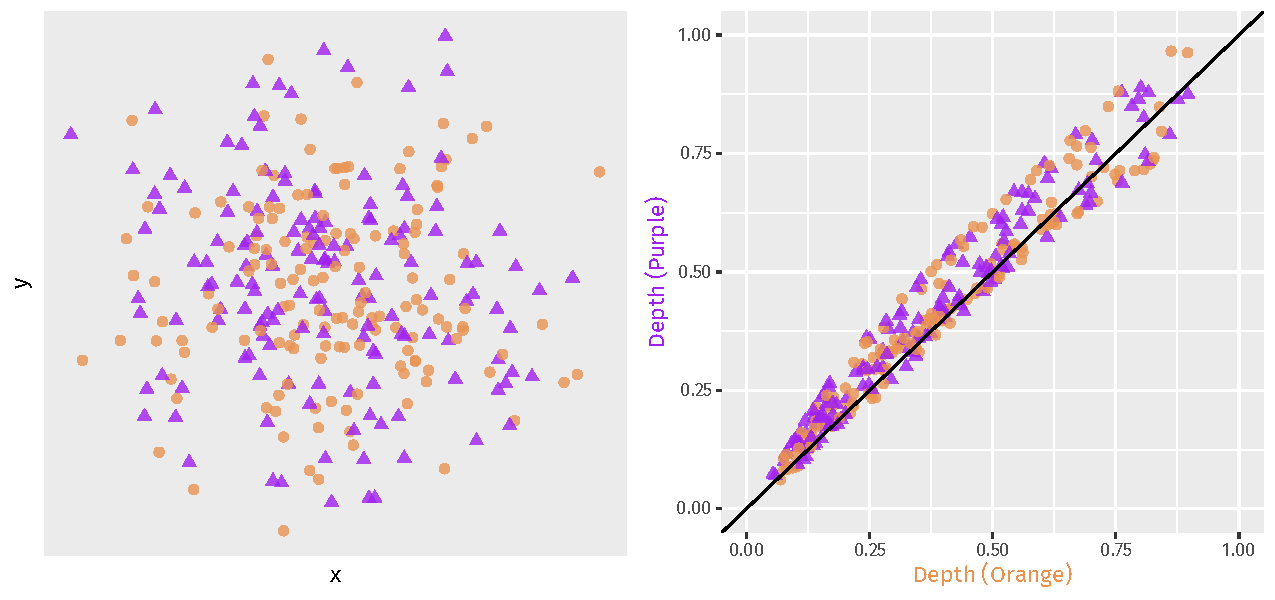
\includegraphics[width = \textwidth, page = 1]{ddplots}
    \caption{
        Empirical DD plot using spatial depth, where both underlying
        distributions (bivariate normal) are identical.
        Observe how the points in the DD plot stay close to the diagonal black
        line.
    }
    \label{fig:ddplots_identical}
\end{figure}



If the distributions $F, G$ are unknown, we may use data samples
$\mathscr{D}_F = \{\vX_i\}$ and $\mathscr{D}_G = \{\vY_j\}$ where $\vX_1,
\dots, \vX_n \iid F$ and $\vY_1, \dots, \vY_m \iid G$, then construct
empirical distributions $\hat{F}_n, \hat{G}_m$.
With this, we may examine the empirical DD plot
\begin{equation}
    \DD(\hat{F}_n, \hat{G}_n) \,=\, \{(D(\vz, \hat{F}_n), D(\vz, \hat{G}_m)) : \vz \in \mathscr{D}_F \cup \mathscr{D}_G\}.
\end{equation}

DD plots can be used as a diagnostic tool to detect differences in location
and scale between two multivariate distributions.
\begin{enumerate}[itemsep=0em]
    \item If $F = G$, the points in $\DD(\hat{F}_n, \hat{G}_m)$ stay close to
    the diagonal.
    See Figure~\ref{fig:ddplots_identical}.

    \item If the same point $\vz_0$ achieves maximum depths with respect to
    both distributions $F$ and $G$, this indicates that $\vz_0$ is their
    common center.
    See Figure~\ref{fig:ddplots_location}.

    \item Suppose that $F$ and $G$ have the same center. If the points in
    $\DD(\hat{F}_n, \hat{G}_m)$ arch above the diagonal, i.e.\ the bulk of
    points are deeper in $G$ than in $F$, this indicates that $F$ has a
    greater spread than $G$.
    See Figure~\ref{fig:ddplots_scale_a}.
\end{enumerate}

\textcite{liu-parelius-singh-1999} also demonstrate the use of DD plots to
detect differences in skewness and kurtosis.
This tool is especially convenient since the DD plot is always two dimensional
regardless of the dimension $d$ of the sample points.


\begin{figure}
    \centering
    \includegraphics[width = \textwidth, page = 2]{ddplots}
    \caption{
        Empirical DD plot using spatial depth, where both underlying
        distributions (bivariate normal) differ only in location.
        Observe how most of the orange points fall in the lower triangle,
        while the purple ones fall in the upper triangle.
        The deepest point with respect to the orange distribution has fairly
        low depth with respect to the purple one, and vice versa.
    }
    \label{fig:ddplots_location}
\end{figure}



\begin{figure}
    \centering
    \begin{subfigure}[b]{\textwidth}
        \centering
        \includegraphics[width = \textwidth, page = 3]{ddplots}
        \subcaption{
            $
                \textcolor{Orange}{\Sigma_+} = \I_2, \quad
                \textcolor{Purple}{\Sigma_\times} = 4\I_2,
            $
        }
        \label{fig:ddplots_scale_a}
    \end{subfigure}
    \\[1em]
    \begin{subfigure}[b]{\textwidth}
        \centering
        \includegraphics[width = \textwidth, page = 4]{ddplots}
        \subcaption{
            $
            \textcolor{Orange}{\Sigma_+} = \begin{bmatrix}
                1 & -0.5 \\ -0.5 & 1
            \end{bmatrix}, \quad
            \textcolor{Purple}{\Sigma_\times} = \begin{bmatrix}
                1 & 0.5 \\ 0.5 & 1
            \end{bmatrix}.
            $
        }
        \label{fig:ddplots_scale_b}
    \end{subfigure}
    \\[1em]
    \caption{
        Empirical DD plot using spatial depth, where both underlying
        distributions (bivariate normal) differ only in scale.
        In \textbf{(a)}, observe how the points remain in the upper triangle
        in the DD plot.
        In \textbf{(b)}, observe how there are more orange points in the lower
        triangle, and more purple points in the upper triangle in the DD plot,
        especially in the region close to the origin.
    }
    \label{fig:ddplots_scale}
\end{figure}



\begin{figure}
    \centering
    \includegraphics[width = \textwidth, page = 5]{ddplots}
    \caption{
        Empirical DD plot using spatial depth, where both underlying
        distributions (bivariate normal) differ in both location and scale.
        Observe that there is a clear separation between the orange and purple
        points in the DD plot, although not about the diagonal line.
    }
    \label{fig:ddplots_location_scale}
\end{figure}



\section{Testing}

We are mainly interested in the two sample homogeneity test.
Given samples from $F$ and $G$, we wish to test the null hypothesis $H_0: F =
G$ against an alternate hypothesis that $F$ and $G$ differ in location or
scale.

When $F, G$ are distributions on $\R$, rank based tests such as the Wilcoxon
rank-sum test or the Siegel-Tukey test are readily available.
A very useful tool in this setting is the probability integral transform.

\begin{proposition}
    Let $\vX \sim F$, and let the distribution $F$ be continuous.
    Then, $F(\vX) \sim \UU[0, 1]$.
\end{proposition}

Since $F(\vX_j)$ has the same rank within $\{F(\vX_i)\}$ as does $\vX_j$
within $\{\vX_i\}$, the above result is the key towards establishing many
distribution-free tests and procedures.


In the multivariate setting, \textcite{liu-singh-1993} use the following depth
based analogue.

\begin{definition}
    Denote
    \begin{equation}
        R(\vz, F) = P(D(\vX, F) \leq D(\vz, F) \mid \vX \sim F).
    \end{equation}
\end{definition}

Note that in the empirical setting, $R(\vz, \hat{F}_n)$ is simply the
proportion of sample points $\{\vX_i\}$ which are deeper in $F$ than $\vz$.


\begin{proposition}[\cite{liu-singh-1993}]
    Let $\vX \sim F$, and let the distribution of $D(\vX, F)$ be continuous.
    Then, $R(\vX, F) \sim \UU[0, 1]$.
\end{proposition}


\begin{definition}
    Denote the quality index
    \begin{equation}
        Q(F, G) = P(D(\vX, F) \leq D(\vY, F) \mid \vX \sim F,\, \vY \sim G).
    \end{equation}
\end{definition}

Note that $Q(F, G)$ and $Q(G, F)$ are not necessarily the same.
We may also write
\begin{equation}
    Q(F, G) = \E_{\vY \sim G}[R(\vY, F)].
\end{equation}


It is clear that $Q(F, G) = 1/2$ when $F = G$.
It can be shown under special circumstances that $Q(F, G) < 1/2$ if $F, G$
differ in terms of location or scale.
This will form the basis of our testing scheme, with $H_0: F = G$ versus $H_A:
Q(F, G) < 1/2$.

Here, we restrict our attention to elliptical distributions on $\R^d$.

\begin{definition}[Elliptical distributions]
    We say that a distribution is elliptical if it has a density of the form
    \begin{equation}
        f(\vx) = c\, |\Sigma|^{-1/2}\, h\left((\vx - \vmu)^\top \Sigma^{-1} (\vx - \vmu)\right)
    \end{equation}
    for some non-increasing function $h$.
    This is denoted by $\Ell(h; \vmu, \Sigma)$.
\end{definition}

% \begin{proposition}[\cite{liu-singh-1993}]
%     Let $F \sim \Ell(h; \vmu, \Sigma)$ and $G_t \sim \Ell(h; \vmu +
%     t\hat{\vv}, \Sigma)$ for some unit vector $\hat{\vv}$ and $t \geq 0$.
%     Further suppose that $D(\cdot, F)$ has the affine invariance and
%     monotonicity properties.
%     Then, $Q(F, G_t)$ is non-increasing with increasing $t$.
% \end{proposition}

% \begin{proposition}[\cite{liu-singh-1993}]
%     Let $F \sim \Ell(h; \vmu, \Sigma_1)$ and $G \sim \Ell(h; \vmu, \Sigma_2)$
%     where $\Sigma_1 - \Sigma_2$ is positive definite.
%     Further suppose that $D(\cdot, F)$ has the affine invariance property.
%     Then, $Q(F, G) \leq 1/2$.
% \end{proposition}

The quality index obeys the following properties.

\begin{proposition}[\cite{liu-singh-1993}]
    Let $F \sim \Ell(h; \vmu_1, \Sigma_1)$ and $G \sim \Ell(h; \vmu_2,
    \Sigma_2)$ where $\Sigma_1 - \Sigma_2$ is positive definite.
    Further suppose that $D(\cdot, F)$ has the affine invariance and
    monotonicity properties.
    Then, $Q(F, G) \leq 1/2$ decreases monotonically as $\vmu_2$ is moved away
    from $\vmu_1$ along any line.
\end{proposition}

\begin{proposition}[\cite{liu-singh-1993}]
    Let $F \sim \Ell(h; \vmu, \Sigma_1)$ and $G \sim \Ell(h; \vmu,
    \Sigma_2)$ where $\Sigma_1 - \Sigma_2$ is positive definite.
    Consider Huber's contamination of the form
    \begin{equation}
        G_\alpha = (1 - \alpha)F + \alpha G
    \end{equation}
    where $0 \leq \alpha \leq 1$.
    Then, $Q(F, G_\alpha)$ decreases monotonically as $\alpha$ increases.
\end{proposition}

This motivates a modified Wilcoxon rank-sum test in the multivariate setting,
using the quality index $Q(F, G)$.
Let $\vX_1, \dots, \vX_n \iid F$, and $\vY_1, \dots, \vY_m \iid G$.
Since $R(\cdot, F), Q(F, \cdot)$ depend on $D(\cdot, F)$, the latter has to be
approximated using $D(\cdot, \hat{F}_{n_0})$, where $\hat{F}_{n_0}$ is based
on a (fairly large) additional sample $\vZ_1, \dots, \vZ_{n_0} \iid F$, with
$n_0 \gg n, m$.
With this, we compute
\begin{equation}
    R(\,\cdot\,, \hat{F}_{n_0}) = \frac{1}{n_0} \sum_{i = 1}^{n_0} \bm{1}(D(\vZ_i, \hat{F}_{n_0}) \leq D(\,\cdot\,, \hat{F}_{n_0})).
\end{equation}
Assign ranks $1, \dots, n + m$ to the arranged values $R(\vX_i,
\hat{F}_{n_0}), R(\vY_j, \hat{F}_{n_0})$ (ascending order), and define $W$ to
be the sum of ranks of the $R(\vY_j, \hat{F}_{n_0})$.
If necessary, break ties at random.
Under the null hypothesis $F = G$, it is clear that $W$ has the same
distribution as the sum of $m$ numbers drawn without replacement from $\{1,
\dots, n + m\}$.
Under the alternate hypothesis $Q(F, G) < 1/2$, the ranks of $R(\vY_j,
\hat{F}_{n_0})$ will tend to be lower on average, making $W$ smaller.

\begin{theorem}[\cite{liu-singh-1993}]
    Let $H_{n, m}$ be the distribution of the sum of $m$ numbers drawn
    randomly without replacement from $\{1, \dots, n + m\}$.
    Suppose that $F$ admits a density function $f$.
    Under the null hypothesis $F = G$, we have $W \sim H_{n, m}$.
\end{theorem}

It is also possible to approximate $Q(F, G)$ more directly via $Q(\hat{F}_n,
\hat{G}_m)$ and perform our test this way.
This sidesteps the need for the `reference' sample $\vZ_1, \dots, \vZ_{n_0}
\iid F$.
Note that
\begin{equation}
    Q(\hat{F}_n, \hat{G}_m)
    = \frac{1}{m}\sum_{j = 1}^m R(\vY_j, \hat{F}_n)
    = \frac{1}{nm}\sum_{i, j} \bm{1}(D(\vX_i, \hat{F}_n) \leq D(\vY_j, \hat{F}_n)).
\end{equation}
This estimate is indeed consistent under mild assumptions.

\begin{theorem}[\cite{liu-singh-1993}]
    Suppose that the distribution of $D(\vY, F)$ is continuous where $\vY \sim
    G$, and that
    \begin{equation}
        \sup_{\vz \in \R^d} |D(\vz, \hat{F}_n) - D(\vz, F)| \toas 0.
    \end{equation}
    Then, $Q(\hat{F}_n, \hat{G}_n) \toas Q(F, G)$ as $\min\{n, m\} \to
    \infty$.
\end{theorem}

This allows us to determine the asymptotic null distribution of $Q(\hat{F}_n,
\hat{G}_m)$.

\begin{theorem}[\cite{liu-singh-1993}]
    Let $F$ be absolutely continuous, such that $\E_{\vX \sim F} \norm{\vX}^4
    < \infty$.
    Using Mahalanobis depth to define $Q$, we have
    \begin{equation}
        S(\hat{F}_n, \hat{G}_m) = \left[\frac{1}{12}\left(\frac{1}{n} + \frac{1}{m}\right)\right]^{-1/2} \left[Q(\hat{F}_n, \hat{G}_m) - \frac{1}{2}\right] \tod \NN(0, 1)
    \end{equation}
    as $\min\{n, m\} \to \infty$, under the null hypothesis $F = G$.
\end{theorem}

Observe that given two samples, we have a choice between using $Q(\hat{F}_n,
\hat{G}_m)$ or $Q(\hat{G}_m, \hat{F}_n)$.
\textcite{shi-zhang-fu-2023} propose a weighted combination of the form
\begin{equation}
    W^\alpha_{n, m} = \alpha S(\hat{F}_n, \hat{G}_m)^2 + (1 - \alpha) S(\hat{G}_m, \hat{F}_n)^2
\end{equation}
for $\alpha \in [0, 1]$, or a maximum
\begin{equation}
    M_{n, m} = \max\{S(\hat{F}_n, \hat{G}_m)^2, S(\hat{G}_m, \hat{F}_n)^2\}.
\end{equation}
Under similar assumptions, they show that both $W^\alpha_{n, m} \tod \chi^2_1$
and $M_{n, m} \tod \chi^2_1$ as $\min\{n, m\} \to \infty$ and $n / m$
converges to a positive constant, under the null hypothesis $F = G$.


\section{Classification}
\label{ch:multivariate_classification}

The $k$-class classification task involves assigning an observation $\vx$ to
one of $k$ populations, described by distributions $F_i$ for $1 \leq i \leq
k$.
The populations may also be associated with prior probabilities $\pi_i$.

\begin{definition}[Classifier]
    A classifier is a map $\hat{\iota}\colon \R^d \to \{1, \dots, k\}$.
\end{definition}

\begin{example}[Bayes classifier]
    Suppose that the population densities $f_i$ for each $1 \leq i \leq k$ are
    known.
    The Bayes classifier assigns $\vx$ to the $\hat{\iota}_B$-th population
    where
    \begin{equation}
        \hat{\iota}_B(\vx) \,=\, \argmax_{1 \leq i \leq k}\; \pi_i f_i(\vx).
    \end{equation}
\end{example}

One way of measuring the performance of a classifier (given the population
distributions and their priors) is by measuring its average misclassification
rate.

\begin{definition}[Average misclassification rate]
    The average misclassification rate of a classifier $\hat{\iota}$ is given
    by
    \begin{equation}
        \Delta(\hat{\iota}) \,=\, \sum_{i = 1}^k \pi_i P(\hat{\iota}(\vX) \neq i \mid \vX \sim F_i).
    \end{equation}
\end{definition}

\begin{proposition}
    The Bayes classifier has the lowest possible average misclassification
    rate. This is known as the optimal Bayes risk, denoted $\Delta_B$.
\end{proposition}

The simplest depth based classifier is the maximum depth classifier
\parencite{ghosh-chaudhuri-2005}.

\begin{example}[Maximum depth classifier]
    Suppose that the prior probabilities $\pi_i$ are equal.
    The maximum depth classifier $\hat{\iota}_D$ for a choice of depth
    function $D$ is described by
    \begin{equation}
        \hat{\iota}_D(\vx) \,=\, \argmax_{1 \leq i \leq k}\; D(\vx, F_i).
    \end{equation}
\end{example}

In practice, instead of having direct access to the population distributions
$F_i$, we have typically deal with labeled training data
\begin{equation}
    \mathscr{D} \,=\, \{(\vx_{ij}, i)\} \subset \R^d \times \{1, \dots, k\},
\end{equation}
where $\vx_{i1}, \dots, \vx_{in_i} \iid F_i$ for each $1 \leq i \leq k$.
The empirical maximum depth classifier simply replaces the population
distributions $F_i$ with their empirical counterparts $\hat{F}_i$ determined
by $\vx_{i1}, \dots, \vx_{in_i}$. Thus, it is given by
\begin{equation}
    \hat{\iota}_{D}(\vx) \,=\, \argmax_{1 \leq i \leq k}\; D(\vx, \hat{F}_i).
\end{equation}
Under certain restrictions, this classifier becomes asymptotically optimal in
the following sense.

\begin{theorem}[\cite{ghosh-chaudhuri-2005}]
    Suppose that the population density functions $f_i$ are elliptically
    symmetric, with $f_i(\vx) = g(\vx - \vmu_i)$ for parameters $\vmu_i$ and a
    density function $g$ such that $g(k\vx) \leq g(\vx)$ for every $\vx$ and
    $k > 1$. Further suppose that the priors on the populations are equal, and
    the depth function $D$ is one of HD, SD, MJD, PD. Then,
    $\Delta(\hat{\iota}_{D}) \to \Delta_B$ as $\min\{n_1, \dots,
    n_k\} \to \infty$.
\end{theorem}

Note that this result deals with elliptic population densities differing only
in location.
Relax this assumption, and instead suppose that $f_i \sim \Ell(h_i; \vmu_i,
\Sigma)$, i.e.
\begin{equation}
    f_i(\vx) = c_i |\Sigma|^{-1/2} h_i\left((\vx - \vmu_i)^\top \Sigma^{-1} (\vx - \vmu_i)\right)
\end{equation}
for strictly decreasing $h_i$, and that the depths can be expressed as
$D(\Cdot, F_i) = l_i(f_i(\Cdot))$ for strictly increasing functions $l_i$.
It follows that the Bayes decision rule can be reformulated as
\begin{equation}
    \pi_i f_i(\vx) > \pi_j f_j(\vx) \;\iff\; D(\vx, F_i) > r_{ij}(D(\vx, F_j))
\end{equation}
for some real increasing function $r_{ij}$.
Using this observation, the DD classifier \parencite{li-albertos-liu-2012}
picks separating functions $r_{ij}$ which best classify the training data
$\mathscr{D}$.

\begin{definition}[Empirical misclassification rate]
    The empirical misclassification rate of a classifier $\hat{\iota}$, with
    respect to data $\mathscr{D}$, is given by
    \begin{equation}
        \hat{\Delta}(\hat{\iota}) \,=\, \sum_{i = 1}^k \frac{\pi_i}{n_i}\sum_{j = 1}^{n_i} \bm{1}(\hat{\iota}(\vx_{ij}) \neq i).
    \end{equation}
\end{definition}


\begin{definition}[DD classifier]
    Suppose that $k = 2$, that $D$ is a depth function, and that $r\colon [0,
    1] \to [0, 1]$ is an increasing function. The DD classifier
    $\hat{\iota}_{D, r}$ is given by
    \begin{equation}
        \hat{\iota}_{D, r}(\vx) \,=\, \begin{cases}
            1, &\text{ if } D(\vx, F_2) \leq r(D(\vx, F_1)), \\
            2, &\text{ if } D(\vx, F_2) >    r(D(\vx, F_1)).
        \end{cases}
    \end{equation}
    % The optimal separating curve $r$ is chosen from a family of curves
    % $\Gamma$ so as to minimize the average classification error, i.e.\ \[
    %     r = \argmin_{r' \in \Gamma} \Delta(\hat{\iota}_{D, r'}).
    % \]
    The empirical DD classifier $\hat{\iota}_{D, \hat{r}}$ replaces $F_i$ by
    their empirical counterparts $\hat{F}_i$.
    Here, the separating curve $\hat{r}$ is chosen from a family $\Gamma$ so
    as to minimize the empirical misclassification rate, i.e.
    \begin{equation}
        \hat{r} = \argmin_{r \in \Gamma} \hat{\Delta}(\hat{\iota}_{D, r}).
    \end{equation}
\end{definition}
\begin{remark}
    The maximum depth classifier $\hat{\iota}_D$ is simply the DD classifier
    $\hat{\iota}_{D, \id}$, where $\id(x) = x$.
    Figure~\ref{fig:ddplots_location_scale} clearly illustrates how this
    choice of separating function may not always be appropriate.
\end{remark}

\textcite{li-albertos-liu-2012} show that under certain restrictions, the
empirical DD classifier is asymptotically equivalent to the Bayes rule. We
give one such instance below.

\begin{lemma}
    Suppose that the following conditions hold.
    \vspace{-1em}
    \begin{enumerate}[itemsep = -0.2em]
        \item $\Gamma$ is the class of polynomial functions on $[0, 1]$.
        \item The depth functions $D(\Cdot, F_i)$ are continuous.
        \item As $\min\{n_1, n_2\} \to \infty$, we have for each $i \in \{1, 2\}$,
        \begin{equation}
            \sup_{\vz \in \R^d} |D(\vz, \hat{F}_i) - D(\vz, F_i)| \toas 0.
        \end{equation}
        \item The distributions $F_i$ are elliptical and satisfy for all
        $\delta \in \R$
        \begin{equation}
            P(D(\vZ, F_i) = \delta \mid \vZ \sim F_i) = 0.
        \end{equation}
    \end{enumerate}
    Then, $\Delta(\hat{\iota}_{D, \hat{r}}) \to \Delta_B$ as $\min\{n_1, n_2\}
    \to \infty$.
\end{lemma}

In all the depth based classifiers we have seen so far, the classification
rule depends on the observation $\vx$ only through the depths $D(\vx, F_i)$.
Thus, we are motivated to define the following transformation from $\R^d$ to a
depth feature space.

\begin{definition}
    The depth feature vector $\vx^D$ of an observation $\vx$, with respect to
    the population distributions $F_i$ and a choice of depth function $D$, is
    defined as
    \begin{equation}
        \vx^D \,=\, \left(D(\vx, F_1), \dots, D(\vx, F_k)\right).
    \end{equation}
\end{definition}
\begin{remark}
    The graph
    \begin{equation}
        \DD(F_1, \dots, F_k) = \{\vx^D : \vx \in \R^d\}
    \end{equation}
    is the analogue of the \nameref{def:ddplot}, with $k$ distributions.
\end{remark}

Assuming that the depth function $D$ only takes values in $[0, 1]$, the map
$\vx \mapsto \vx^D$ takes values in $[0, 1]^k$, regardless of the
dimensionality of the original vector $\vx$.
With this, the maximum depth classification rule can be expressed as
\begin{equation}
    \hat{\iota}_D(\vx) = i \;\iff\; \vx^D \in R_i^D = \{\vy \in [0, 1]^k : y_i = \max_j y_j\}.
\end{equation}
Indeed, any partition of the unit cube $[0, 1]^k$ into $k$ decision regions
$R^D_i$ gives rise to a depth based classifier.
The DD classifier achieves this by using an increasing separating function
$r$ to partition $[0, 1]^2$.
Furthermore, $r \in \Gamma$ is chosen so as to best separate the training data
$\mathscr{D}$ transformed into the depth feature space.
However, we can in principle use the transformed training data
\begin{equation}
    \mathscr{D}^D \,=\, \{(\vx^D_{ij}, i)\} \subset [0, 1]^k \times \{1, \dots, k\}
\end{equation}
along with any multivariate classification algorithm (LDA, QDA, $k$NN, GLM,
etc) to devise suitable decision regions.
This is the basis of the DD$^G$ classifier
\parencite{albertos-bande-fuente-2017}.




\section{Clustering}

The unsupervised clustering grouping a collection of observations, such that
points within the same group are more similar to each other than those from
different groups.

\begin{definition}[Clustering]
    Given observations $\vx_1, \dots, \vx_N \in \R^d$, a clustering assignment
    is a choice of a partition $I_1, \dots, I_K$ of $\{1, \dots, N\}$.
\end{definition}

With this notation, the $k$-th cluster consists of the points $\{\vx_i\}_{i
\in I_k}$.
A good cluster assignment is one that maximizes similarity within clusters, as
well as dissimilarity between clusters.
Thus, the problem of clustering can be framed as the optimization of some
objective function which combines these notions of similarity and
dissimilarity.
A simple algorithm such as the $K$-means clustering seeks to minimize
\begin{equation}
    \{I_1, \dots, I_K\} \mapsto \frac{1}{N} \sum_{k = 1}^K \sum_{i \in I_k} \norm{\vx_i - \vmu_k}^2,
\end{equation}
the average sum of square distances between each point and its cluster mean
\begin{equation}
    \vmu_k = \frac{1}{|I_k|} \sum_{i \in I_k} \vx_i
    = \argmin_{\vmu \in \R^d} \sum_{i \in I_k} \norm{\vx_i - \vmu}^2.
\end{equation}
\textcite{jornsten-2004} proposes a depth based approach to this problem, by
examining the depth of a point within its cluster, relative to its depth
within the best competing cluster.

In this section, we will abbreviate $D_k(\vx) = D(\vx, \hat{F}_{I_k})$, i.e.\
the empirical depth of $\vx$ with respect to the points in the $k$-th cluster.
\textcite{jornsten-2004} chooses $L_1$ depth, the empirical version of spatial
depth.

\begin{definition}
    The within cluster depth of $\vx_i$ is $D_i^w = D_k(\vx_i)$, where $i \in
    I_k$.
\end{definition}

To deal with dissimilarity between clusters, we represent each cluster by its
$L_1$-median.

\begin{definition}[$L_1$-median]
    The $L_1$-median of the $k$-th cluster is given by
    \begin{equation}
        \vth_k = \argmin_{\vth \in \R^d} \sum_{i \in I_k} \norm{\vx_i - \vth}.
    \end{equation}
\end{definition}

\begin{definition}
    The between cluster depth of $\vx_i$ is $D_i^b = D_\ell(\vx_i)$, where
    \begin{equation}
        \ell = \argmin_{k \colon i \notin I_k} \norm{\vx_i - \vth_k}.
    \end{equation}
\end{definition}

In other words, the between cluster depth of $\vx_i$ is its depth within the
best competing cluster.

\begin{definition}[Relative depth]
    The relative depth of $\vx_i$ is $\ReD_i = D_i^w - D_i^b$.
\end{definition}

A point $\vx_i$ is \emph{well clustered} if $\ReD_i$ is very high, i.e.\ it is
deep within its own cluster, and has low depth with respect to its next best
competing cluster.
Thus, to obtain a good clustering, we may choose to maximize the objective
function
\begin{equation}
    \{I_1, \dots, I_K\} \,\mapsto\, \frac{1}{N} \sum_{k = 1}^K \sum_{i \in I_k} \ReD_i,
\end{equation}
which is simply the average relative depth.
This maximization can be achieved iteratively, starting with a random cluster
assignment and reassigning a subset of observations with low $\ReD_i$ to their
nearest competing clusters.
The reassignment is accepted if the objective function increases, and the
process is repeated.
\textcite{jornsten-2004} also suggests the use of simulated annealing to
overcome the problem of getting trapped in local maxima.
Here, the reassignment is accepted with some probability $P(\beta, \delta)$
where $\delta$ is the change in the objective function value, even if the
objective function decreases at that step.
$P(\beta, \delta)$ is chosen to decrease with increasing $\beta$ and $\delta$.
The tuning parameter $\beta$ can be increased every iteration so that the
probability of accepting poorer clustering assignments drops to zero
eventually.

Another notion of similarity and dissimilarity involves \emph{silhouette
width}.

\begin{definition}[Silhouette width]
    Denote the average distance of $\vz$ from points in the $k$-th cluster not
    equal to $\vz$ by
    \begin{equation}
        \bar{d}_k(\vz) = \frac{1}{|\{i \in I_k\colon \vx_i \neq \vz\}|} \sum_{\stackrel{i \in I_k}{\vx_i \neq \vz}} \norm{\vx_i - \vz}.
    \end{equation}
    The silhouette width of $\vx_i$ where $i \in I_k$ is given by
    \begin{equation}
        \Sil_i = \frac{b_i - a_i}{\max\{a_i, b_i\}}, \qquad
        a_i = \bar{d}_k(\vx_i), \quad
        b_i = \min_{\ell \neq k} \bar{d}_\ell(\vx_i).
    \end{equation}
\end{definition}

It has been observed that the silhouette width is greatly affected by
differences in scale between clusters, while the relative depth is not.
An objective function of the form
\begin{equation}
    \{I_1, \dots, I_K\} \,\mapsto\, \frac{1}{N} \sum_{k = 1}^K \sum_{i \in I_k} (1 - \lambda)\Sil_i + \lambda\ReD_i
\end{equation}
may be used to combine both notions.
Here, $\lambda \in [0, 1]$ controls the influence of the relative depth.
It seems that small values of $\lambda$ encourages equal scale clusters, while
large values of $\lambda$ allows unequal scale clusters.
Thus, $\lambda$ may be tuned accordingly to favour these different kinds of
clustering assignments.


\section{Outlier detection}
